\chapter{Уравнения в системе координат, связанных с давлением}

\section{{\color{done}Локальные декартовы координаты}}

    В качестве отправной точки выпишем заново систему уравнений Навье-Стокса в декартовых координатах для случая идеальной жидкости и условия гидростатичности (уравнения (\ref{eq:DuDt_geost})-(\ref{eq:DthetaDt})), подразумевая тем самым, что речь будет идти об уравнениях, пригодных для моделирования крупномасштабных атмосферных процессов. Эту систему дополним уравнением состояния.

    \begin{equation}
    \label{eq:ch6-DuDt_geost}
        \td{u}{t} = -\frac{1}{\rho}\pd{p}{x}+fv 
    \end{equation} 
    \begin{equation}
    \label{eq:ch6-DvDt_geost}
        \td{v}{t} = -\frac{1}{\rho}\pd{p}{y}-fu 
    \end{equation} 
    \begin{equation}
    \label{eq:ch6-DzDt_geost}
        0 = -\frac{1}{\rho}\pd{p}{z}-g 
    \end{equation} 
    \begin{equation}
    \label{eq:ch6-masscons}
        \pd{\rho}{t} + \pd{(\rho u)}{x} + \pd{(\rho v)}{y} + \pd{(\rho w)}{z} = 0 
    \end{equation} 
    \begin{equation}
    \label{eq:ch6-Tcons} % ЗАЛОЖЕНА ОШИБКА
        \pd{\theta}{t} + \pd{\theta}{x} + \pd{\theta}{y} + \pd{\theta}{z} = \varepsilon\frac{\theta}{T} \frac{1}{\rho c_p} 
    \end{equation} 
    \begin{equation}
        \label{eq:ch6-idealGas}
        p = R\rho T
    \end{equation} 

    Недостатком системы (\ref{eq:ch6-DuDt_geost})-(\ref{eq:ch6-idealGas}) является большое количество нелинейных членов как в правых, так и в левых частях уравнений. Ситуация может быть несколько облегчена, если в качестве вертикальной координаты использовать давление. В $z$-системе координат в уравнениях (\ref{eq:ch6-DuDt_geost})-(\ref{eq:ch6-idealGas}) члены с давлением в общем случае сжимаемой жидкости являются нелинейными, равно как и три члена в уравнении сохранения массы. Оказывается, что если воспользоваться в качестве вертикальной координаты не геометрической высотой, а давлением, то члены с давлением в уравнении движения и уравнение неразрывности становятся линейными. Это существенно упрощает исходную систему, поэтому уравнения в $p$-системе координат, а вернее в некоторых производных от $p$-системы координат, широко используются как в исследовательских, так и в прогностических моделях атмосферы. Так как в атмосфере доминирует условие гидростатики, давление монотонно падает с высотой. Это свойство монотонности очень важно. Например, потенциальная температура, которая во многом является также удачной вертикальной координатой, используется гораздо реже, т.к. в изентропических координатах не гарантируется монотонный рост $\theta$ с высотой: в условиях неустойчивой стратификации $\theta$ с высотой падает, а знакопеременная координата крайне неудобна для анализа.

    Итак, в изобарической системе координат горизонтальные координаты остаются прежними, а изменяется только вертикальная координата. Для начала мы тем не менее введем для горизонтальных координат обозначения $x_p, y_p$ и будем иметь дело с $f(x_p,y_p,p,t_p)$. Таким образом задача заключается в переходе от  $f(x,y,z,t)$ к этим новый координатам с наложением дополнительных условий: $x_p=x,y_p=y$ и $t_p=t)$.

    \begin{figure}[h]
    \centering
    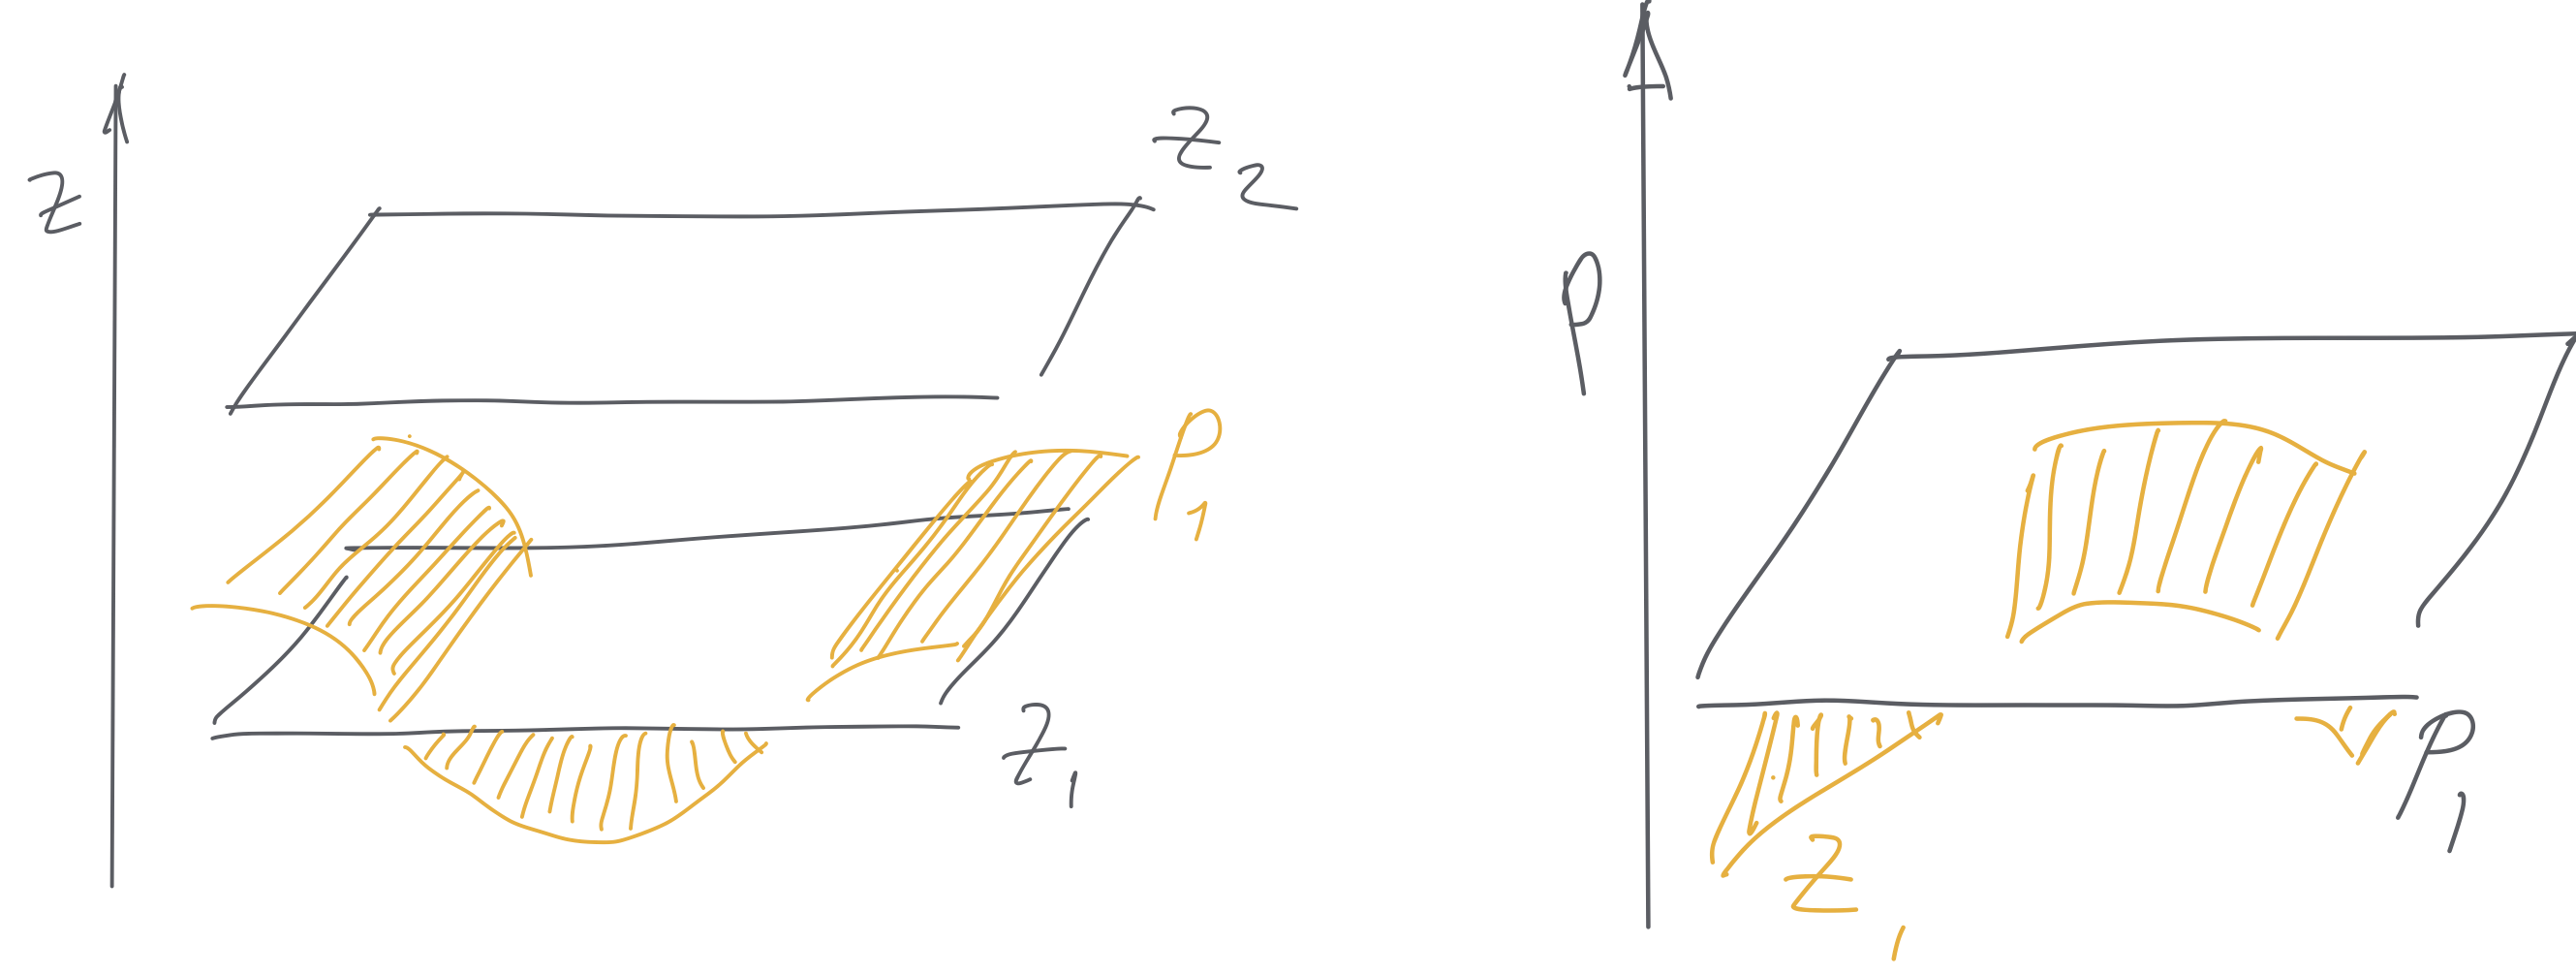
\includegraphics[width=0.9\linewidth]{pics/ch6.1.png}
    \caption{\label{fig:ch6.1}
    Схематичное пояснение систем координат. $p$-поверхность в $z$-системе координат (слева) и $z$-поверхность в $p$-системе координат
    }
    \end{figure}    

    Система координат $(x,y,p)$ является ортогональной декартовой системой координат. Высота изобарической поверхности $h(x,y,p,t)$ становится зависимой переменой в новой системе. Если мы будем смотреть на изобарические их ортогональной системы $(x,y,z)$, то они имеют наклон и движутся с течением времени. Но в системе $(x,y,p)$ изобарические поверхности всюду плоские, параллельны друг другу и не движутся. Поле высоты двигается и имеет наклоны, если мы смотрим на него из $p$-системы координат. 

    Горизонтальные компоненты скорости в новой системе координат остаются такими же, как они были в системе $(x,y,z)$, потому что отличия в положении точки измеряются проекцией на плоскость $xy$, а время одно и тоже в обеих системах. Вертикальная скорость изменяется отличием $p$ от $z$.

    Соотношение между $p$ и $z$ нам дает уравнение гидростатики, поэтому переход между этими системами возможен только в случае условия гидростатичности. В качестве функций в новой системе координат будут: $u,v,\tau$, точно такие же, как и в $z$-системе, высота изобарической поверхности $H$ и функция 
    \begin{equation}
        \label{eq:tau}
        \tau=\fd{p},
    \end{equation}
    которая является аналогом вертикальной скорости в $p$-системе координат. Для более ясного понимания $\tau$ сохраним в нем последний, наиболее большой член. Тогда будем иметь $\tau\simeq w\pd{p}{z}=-w\rho g$ [кг/(мс$^3$)] или [кг/(мс$^2$с)=гПа/с]. Из знака правой части последнего соотношения следует, что $\tau>0$ при $w<0$ и наоборот.

    Чтобы записать систему (\ref{eq:ch6-DuDt_geost})-(\ref{eq:ch6-idealGas}) в изобарической системе координат, необходимо произвести замену переменных в дифференциальных уравнениях. Для этого нужно воспользоваться правилом дифференцирования сложных функций:

    \begin{equation}
        \label{eq:ch6-diffrule}
        \pd{f}{\zeta}=\pd{f}{x}\pd{x}{\zeta}+\pd{f}{y}\pd{y}{\zeta}+\cdots+\pd{f}{t}\pd{t}{\zeta}.
    \end{equation}
    Нашими операторами, которые предстоит заменить, являются $\pd{}{x},\pd{}{y},\pd{}{z}$ и $\pd{}{t}$. Пользуясь правилом дифференцирования сложной функции (\ref{eq:ch6-diffrule}), выпишем значения этих производных в новых координатах
    \[
    \pd{f}{x}=\pd{f}{x_p}\cancelto{1}{\pd{x_p}{x}}+\pd{f}{y_p}\cancelto{0}{\pd{y_p}{x}}+\pd{f}{p}\pd{p}{x}+\pd{f}{t_p}\cancelto{0}{\pd{t_p}{x}},
    \]
    т.е. т.к. $x_p=x$, то $\pd{x_p}{x}=1$, $y_p$ и $t_p$ от $x$ не зависят, то предыдущее выражение упростится до
    \begin{equation}
        \label{eq:fx2p}
        \pd{f}{x}=\pd{f}{x_p}+\pd{f}{p}\pd{p}{x}.
    \end{equation}
    Далее, отыскиваем производную по $y$
    \[
    \pd{f}{y}=\pd{f}{x_p}\cancelto{0}{\pd{x_p}{y}}+\pd{f}{y_p}\cancelto{1}{\pd{y_p}{y}}+\pd{f}{p}\pd{p}{y}+\pd{f}{t_p}\cancelto{0}{\pd{t_p}{y}},
    \]
    Из равенства $y_p=y$ и независимости $x_p$ и $t_p$ от $y$ имеем
    \begin{equation}
        \label{eq:fy2p}
        \pd{f}{y}=\pd{f}{y_p}+\pd{f}{p}\pd{p}{y}.
    \end{equation}

    \[
    \pd{f}{z}=\pd{f}{x_p}\cancelto{0}{\pd{x_p}{z}}+\pd{f}{y_p}\cancelto{0}{\pd{y_p}{z}}+\pd{f}{p}\pd{p}{z}+\pd{f}{t_p}\cancelto{0}{\pd{t_p}{z}},
    \]
    Из-за независимости $x_p,y_p$ и $t_p$ от $z$ имеем
    \begin{equation}
        \label{eq:fz2p}
        \pd{f}{z}=\pd{f}{p}\pd{p}{z}.
    \end{equation}

    \[
    \pd{f}{t}=\pd{f}{x_p}\cancelto{0}{\pd{x_p}{t}}+\pd{f}{y_p}\cancelto{0}{\pd{y_p}{t}}+\pd{f}{p}\pd{p}{t}+\pd{f}{t_p}\cancelto{1}{\pd{t_p}{t}},
    \]
    Из-за независимости $x_p,y_p$ от $t$ и $t_p=t$ имеем
    \begin{equation}
        \label{eq:ft2p}
        \pd{f}{t}=\pd{f}{t_p}+\pd{f}{p}\pd{p}{t}.
    \end{equation}

    Для преобразования выражений, содержащих переменную $p$, запишем соотношение между старыми и новыми переменными так, чтобы в левых частях стояли производные по новым переменным. Будем иметь
    \[
    \cancelto{0}{\pd{p}{x_p}}=\pd{p}{x}\cancelto{1}{\pd{x}{x_p}}+\pd{p}{y}\cancelto{0}{\pd{y}{x_p}}+\pd{p}{z}\pd{z}{x_p}+\pd{p}{t}\cancelto{0}{\pd{t}{x_p}},
    \]
    а т.к. давление вдоль изобарической поверхности не меняется $\left(\pd{p}{x_p}=0\right)$, $y$ и $t$ от $x_p$ не зависят, предыдущее выражение примет вид
    \begin{equation}
        \label{eq:ch6-px2p}
        0=\pd{p}{x}+\pd{p}{z}\pd{z}{x_p}.
    \end{equation}

    Аналогично, из $\pd{p}{y_p}$ получим
    \begin{equation}
        \label{eq:ch6-py2p}
        0=\pd{p}{y}+\pd{p}{z}\pd{z}{y_p}.
    \end{equation}
    Из $\pd{p}{p}$ получим
    \begin{equation}
        \label{eq:ch6-pz2p}
        1=\pd{p}{z}\pd{z}{p},
    \end{equation}
    а из $\pd{p}{t}$ получим
    \begin{equation}
        \label{eq:ch6-pt2p}
        0=\pd{p}{z}\pd{z}{t_p}+\pd{p}{t},
    \end{equation}
    Пользуясь соотношениями (\ref{eq:ch6-px2p}) - (\ref{eq:ch6-pt2p}) преобразуем уравнение (\ref{eq:ch6-DuDt_geost})
    \begin{multline*} 
        {\overbrace{\pd{u}{t_p}+\pd{u}{p}\pd{p}{t}}^{\pd{u}{t}}}+
        u{\overbrace{\left( \pd{u}{x_p} + \pd{u}{p}\pd{p}{x} \right)}^{\pd{u}{x}}} +
        v{\overbrace{\left( \pd{u}{y_p} + \pd{u}{p}\pd{p}{y} \right)}^{\pd{u}{y}}} + \\
        + w{\underbrace{\left( \pd{u}{p}\pd{p}{z} \right)}_{\pd{u}{z}}} = 
         -\frac{1}{\rho} {\underbrace{\left( -\pd{p}{z}\pd{z}{x_p} \right)}_{\pd{p}{x}}} + fv
    \end{multline*}
    Произведем перегруппировку членов в левой части, а в правой части применим уравнение гидростатики $\left( \pd{p}{z}=-\rho g \right)$ и высоту изобарической поверхности обозначим $z=H$. Получим
    \begin{equation*}
        % \label{eq:ch6-DuDt2p2}
        \pd{u}{t_p}+u\pd{u}{x_p}+v\pd{u}{y_p}+
        \pd{u}{p} {\underbrace{ \left( \fd{p} \right) }_{\tau}} = - g \pd{H}{x_p}+fv.
    \end{equation*}
    Так как выражение в скобках представляет собой $\tau$, будем иметь окончательно
    \begin{equation}
        \label{eq:ch6-DuDt2p}
        \pd{u}{t_p}+u\pd{u}{x_p}+v\pd{u}{y_p}+
        \tau\pd{u}{p} = -g \pd{H}{x_p}+fv.
    \end{equation}
    Нетрудно заметить, что вместо нелинейного члена, описывающего силу градиента давления в $z$-системе координат, аналогичный член в $p$-системе стал линейным.
    Аналогичным образом второе уравнение движения получим в виде 
    \begin{equation}
        \label{eq:ch6-DvDt2p}
        \pd{v}{t_p}+u\pd{v}{x_p}+v\pd{v}{y_p}+
        \tau\pd{v}{p} = - g \pd{H}{y_p}-fu.
    \end{equation}
    Для записи уравнения гидростатики воспользуемся уравнением (\ref{eq:ch6-pz2p}). В результате будем иметь
    \begin{equation}
        \label{ch6:DwDt2p}
        \pd{H}{p}=-\frac{1}{\rho g}=-\frac{RT}{gp}.
    \end{equation}
    Для преобразования уравнения неразрывности запишем его в виде
    \begin{equation*}
        \fd{\rho} + \rho \left( \pd{u}{x} + \pd{v}{y} + \pd{w}{z} \right) = 0.
    \end{equation*}
    Заменяя в нем $\rho$ из уравнения гидростатики $\left( \rho=\frac{1}{g} \pd{p}{z} \right)$, получим
    \begin{equation*}
        \frac{\partial^2 p}{\partial t \partial z} +
        u\frac{\partial^2 p}{\partial x \partial z} +
        v\frac{\partial^2 p}{\partial y \partial z} +
        w\frac{\partial^2 p}{\partial z \partial z} +
        \pd{p}{z} \left( \pd{u}{x} + \pd{v}{y} + \pd{w}{z} \right) = 0.
    \end{equation*}
    Представим 2ой, 3ий и 4ый члены в виде
    \begin{align*}
        u\frac{\partial^2 p}{\partial x \partial z} &= \pd{}{z} \left( u\pd{p}{x} \right) - \pd{u}{z}\pd{p}{x}, \\
        v\frac{\partial^2 p}{\partial y \partial z} &= \pd{}{z} \left( v\pd{p}{y} \right) - \pd{v}{z}\pd{p}{y}, \\
        w\frac{\partial^2 p}{\partial z^2} &= \pd{}{z} \left( w\pd{p}{z} \right) - \pd{w}{z}\pd{p}{z}.
    \end{align*}
    Группируя первые четыре члена
    \begin{align*}
        \pd{}{z} {\underbrace{\left[ \fd{p} \right]}_{\tau}} - \pd{u}{z}\pd{p}{x}-\pd{v}{z}\pd{p}{y}-\pd{w}{z}\pd{p}{z}+\pd{p}{z} \left( \pd{u}{x} + \pd{v}{y} + \pd{w}{z} \right) = 0.
    \end{align*}
   С использование соотношений (\ref{eq:tau}), (\ref{eq:fx2p})--(\ref{eq:fz2p}) имеем
   \begin{multline*}
       \pd{\tau}{z}-
       \cancel{\pd{u}{p}\pd{p}{z}\pd{p}{x}}-
       \cancel{\pd{v}{p}\pd{p}{z}\pd{p}{y}}-
       \cancel{\pd{w}{p}\pd{p}{z}\pd{p}{z}}+ \\
     + \pd{p}{z} \left( \pd{u}{x_p} + \cancel{\pd{u}{p}\pd{p}{x}} + 
     \pd{v}{y_p} + \cancel{\pd{v}{p}\pd{p}{y_p}}+\cancel{\pd{w}{p}\pd{p}{z}} \right) = 0
   \end{multline*}
   Применяя (\ref{eq:fz2p}) к первому члену, получим
   \begin{equation*}
       \pd{\tau}{p}\pd{p}{z} + \pd{p}{z} \left( \pd{u}{x_p} + \pd{v}{y_p} \right) = 0
   \end{equation*}
   или
   \begin{equation*}
       \pd{p}{z} \left( \pd{u}{x_p} + \pd{v}{y_p} + \pd{\tau}{p}  \right) = 0
   \end{equation*}
   Так как $\pd{p}{z}\neq0$, то окончательно имеем
   \begin{equation}
       \pd{u}{x_p} + \pd{v}{y_p} + \pd{\tau}{p} = 0.
   \end{equation}
   Заметим, что уравнение неразрывности в $p$-системе координат стало линейным. Применяя соотношение (\ref{eq:fx2p}) - (\ref{eq:ft2p}) к уравнению притока тепла (\ref{eq:ch6-Tcons}) будем иметь
   \begin{multline*}
        \pd{\theta}{t_p} + 
        \pd{\theta}{p}\pd{p}{t}+u \left( \pd{\theta}{x_p} + \pd{\theta}{p}\pd{p}{x} + \right) + 
        v \left( \pd{\theta}{y_p} + \pd{\theta}{p}\pd{p}{y} + \right) + 
        w \pd{\theta}{p}\pd{p}{z} = \varepsilon\frac{\theta}{T}\frac{1}{\rho c_p}
   \end{multline*}
   С использованием (\ref{eq:tau}) имеем окончательно 
   \begin{equation}
       \label{eq:cp6-Tcons4p}
       \pd{\theta}{t_p} + u\pd{\theta}{x_p} + v\pd{\theta}{y_p} + \tau \pd{\theta}{p} = \varepsilon\frac{\theta}{T}\frac{1}{\rho c_p}
   \end{equation}
   Освободившись теперь от подстрочного индекса $p$ перепишем все полученные уравнения вместе:
   % \begin{multline}
   \begin{align}
        \pd{u}{t}+u\pd{u}{x}+v\pd{u}{y}+\tau\pd{u}{p} &= - g \pd{H}{x}+fv, \label{eq:ch6-DuDt4p} \\
        \pd{v}{t}+u\pd{v}{x}+v\pd{v}{y}+\tau\pd{v}{p} &= - g \pd{H}{y}-fu, \label{eq:ch6-DvDt4p} \\
        \pd{H}{p}=-\frac{1}{\rho g}&=-\frac{RT}{gp}, \label{eq:ch6-DhDp4p}\\
        \pd{u}{x} + \pd{v}{y} + \pd{\tau}{p} &= 0, \label{eq:ch6-masscons4p}\\
        \pd{\theta}{t} + u\pd{\theta}{x} + v\pd{\theta}{y} + \tau \pd{\theta}{p} &= \varepsilon\frac{\theta}{T \rho c_p}. \label{eq:ch6-DthetaDt4p}
   \end{align}
   % \end{multline}
   Достаточно часто вместо геометрической высоты $H$ используется геопотенциал $\Phi=gH$. Тогда уравнение (\ref{eq:ch6-DuDt4p}) - (\ref{eq:ch6-DhDp4p}) приобретает вид
   \begin{align}
        \pd{u}{t}+u\pd{u}{x}+v\pd{u}{y}+\tau\pd{u}{p} &= - \pd{\Phi}{x}+fv, \label{eq:ch6-DuDt4pGeopot} \\
        \pd{v}{t}+u\pd{v}{x}+v\pd{v}{y}+\tau\pd{v}{p} &= -\pd{\Phi}{y}-fu, \label{eq:ch6-DvDt4pGeopot}\\
        \pd{H}{p}=-\frac{1}{\rho g}&=-\frac{RT}{gp}, \label{eq:ch6-DhDp4pGeopot}\\
   \end{align}
   Здесь 
   \begin{equation*}
       \td{}{t}=\pd{}{t}+u\pd{}{x}+v\pd{}{y}+\tau\pd{}{p}.
   \end{equation*}
   Если сравнить уравнения (\ref{eq:ch6-DuDt_geost}), (\ref{eq:ch6-DvDt_geost}) и (\ref{eq:ch6-masscons}) с уравнениями (\ref{eq:ch6-DuDt4p}), (\ref{eq:ch6-DvDt4p}) и (\ref{eq:ch6-masscons4p}), то увидим, что нелинейность в правых частях уравнений движения в $p$-системе исчезли. Аналогично исчезла и нелинейность в уравнении неразрывности.

   Выражение (\ref{eq:tau}) для $\tau$, правая часть которого была записана в $z$-системе координат, можно выразить через геопотенциал. Используя (\ref{eq:ch6-px2p}), (\ref{eq:ch6-py2p}) и (\ref{eq:ch6-pt2p}), получим
   \[
    \tau=-\pd{p}{z}\pd{H}{t_p}-u\pd{p}{z}\pd{H}{x_p}-v\pd{p}{z}\pd{H}{y_p}+w\pd{p}{z}.
   \]
   Исключая отсюда $\pd{p}{z}$ с использование уравнения гидростатики, имеем
   \begin{equation}
       \tau=\rho g \left( \pd{H}{t_p} + u\pd{H}{x_p} + v\pd{H}{y_p} - w \right)
   \end{equation}
   или
   \begin{equation}
       \tau=\rho \left( \pd{\Phi}{t_p} + u\pd{\Phi}{x_p} + v\pd{\Phi}{y_p} - wg \right).
   \end{equation}
   Так как уравнение неразрывности в $p$-системе является линейным, уравнения движения легко записываются в так так называемой дивергентной форме:
   \begin{align}
       \pd{u}{t} + \pd{u^2}{x} + \pd{(uv)}{y}  + \pd{(u \tau)}{p} &= -\pd{\Phi}{x}+lv, \label{eq:ch6-DuDt2p_div} \\
       \pd{v}{t} + \pd{uv}{x}  + \pd{(v^2)}{y} + \pd{(v \tau)}{p} &= -\pd{\Phi}{y}-lu. \label{eq:ch6-DvDt2p_div}
   \end{align}
   \begin{warn}
        Пояснить что такое дивергентная форма уравнений!
   \end{warn}
   \begin{warn}
        Написать кусок, доказывающий эквивалентности этих уравнений на примере эквивалентности уравнения (\ref{eq:ch6-DuDt2p_div}) уравнению (\ref{eq:ch6-DuDt4pGeopot})
   \end{warn}
   Заметим, что в $z$-системе дивергентная форма записи, эквивалентная (\ref{eq:ch6-DuDt2p_div})-(\ref{eq:ch6-DvDt2p_div}) могла бы быть получена только при условии $\rho=const$, то есть только при условии несжимаемости жидкости.
   
   

    
    

\section{Сферические координаты}





